\begin{figure}
    \centering
    \begin{subfigure}{0.3\linewidth}
        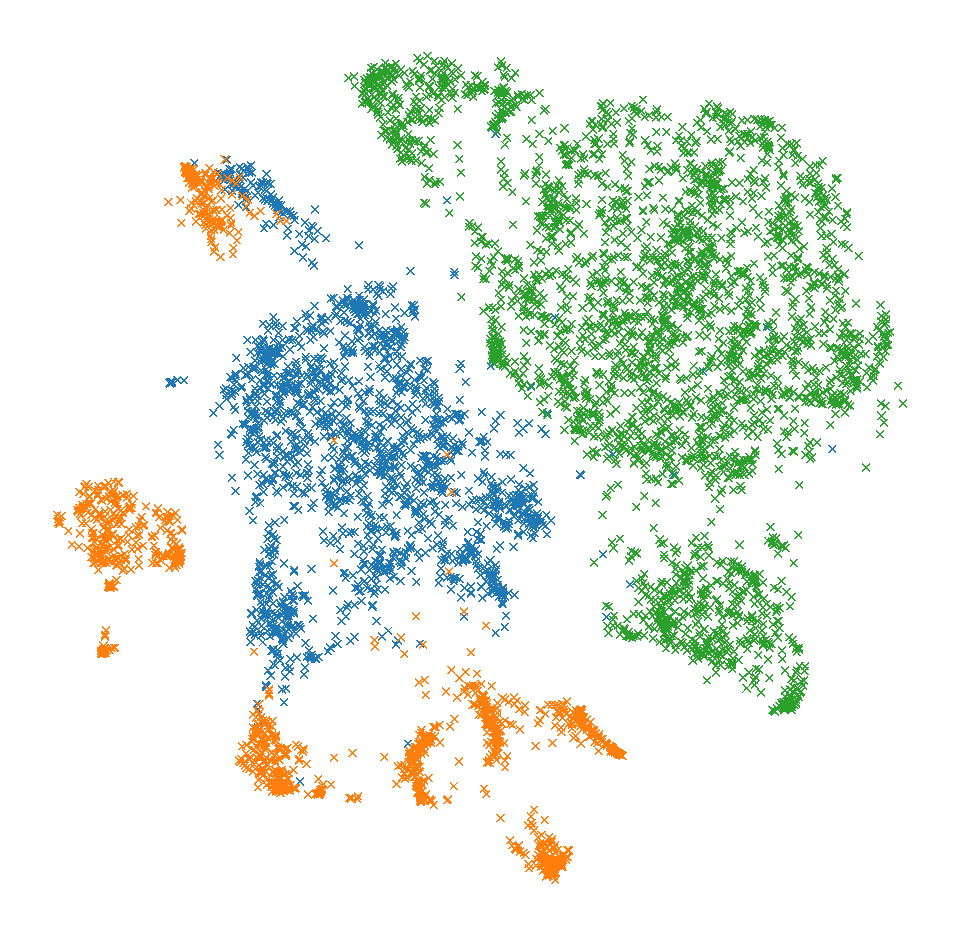
\includegraphics[width=\linewidth]{figures/tsne/PACS_PT.pdf}
        \caption{\small Pre-trained}
        \label{fig:tsne-pretrained}
    \end{subfigure}
    \begin{subfigure}{0.3\linewidth}
        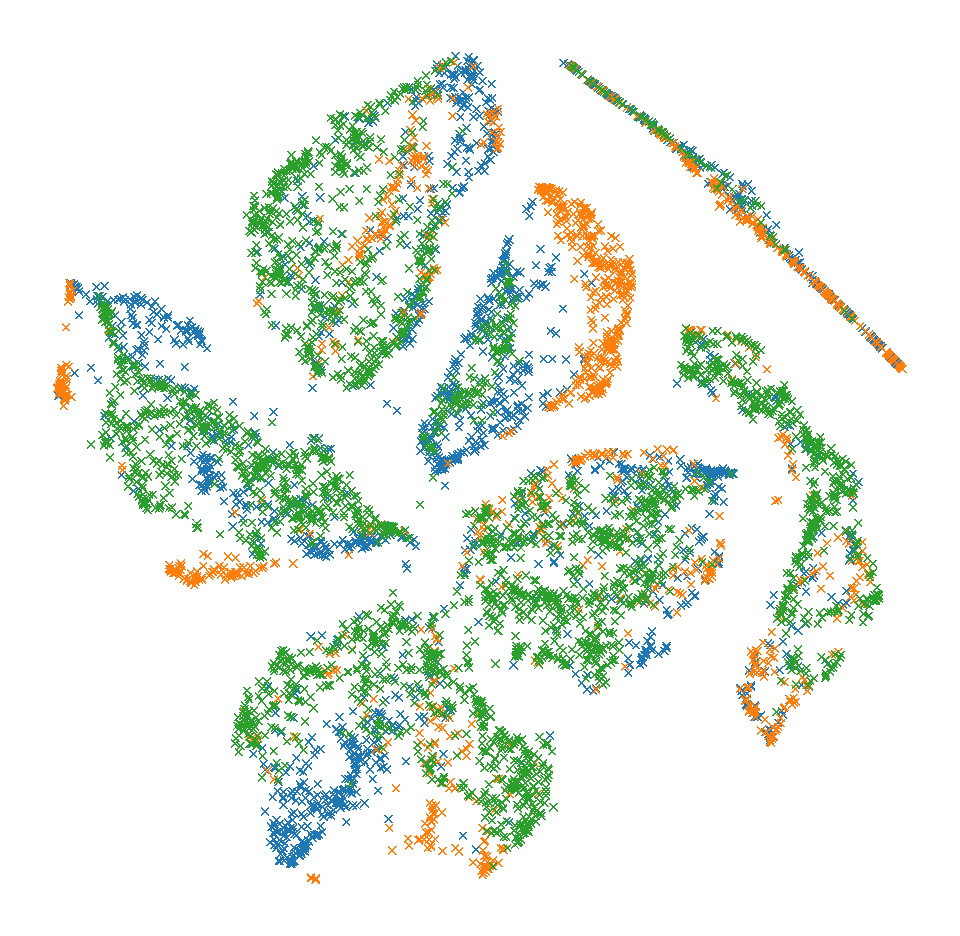
\includegraphics[width=\linewidth]{figures/tsne/PACS_ERM.pdf}
        \caption{\small ERM}
        \label{fig:tsne-erm}
    \end{subfigure}
    % \hfill
    \begin{subfigure}{0.3\linewidth}
        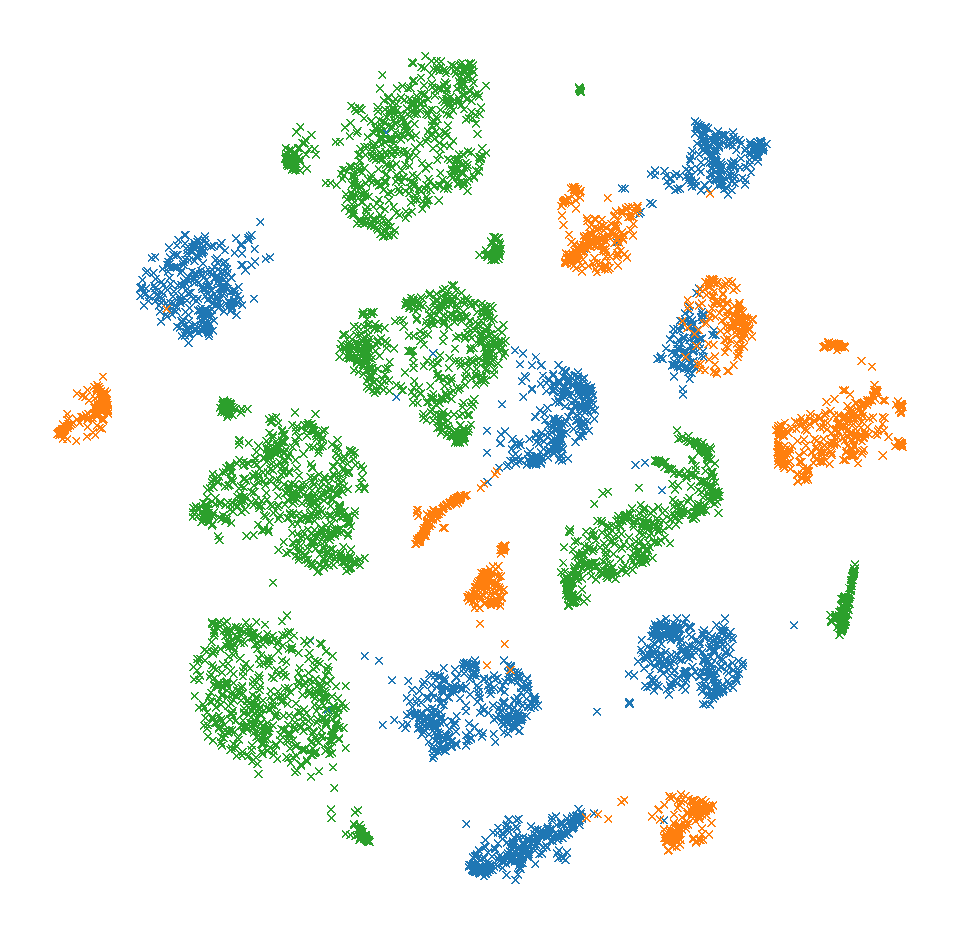
\includegraphics[width=\linewidth]{figures/tsne/PACS_MIRO.pdf}
        \caption{\small MIRO}
        \label{fig:tsne-miro}
    \end{subfigure}
    % \hfill

    \caption{\small \textbf{t-SNE visualization of features in \pacs{}.} Different color indicates different training domain.}
    \label{fig:tsne}
\end{figure}



% \begin{figure}
%     \centering
%     \includegraphics[width=0.7\columnwidth]{figures/mi_all.pdf}
%     \caption{\textbf{Mutual information with oracle model.} \textit{Random} is randomly initialized model, \textit{Scratch} is trained by ERM from \textit{Random}, and \textit{Pretrained} is initialized by pretrained model without training. \textit{ERM} and \textit{SIL} is initialized by pretrained model and trained by each method. $\dagger$ indicates RegNetY-16GF pretrained by SWAG is used and ResNet-50 pretrained in ImageNet is used for the others.}
%     \label{fig:mi}
% \end{figure}



